\documentclass[SKL-MASTER.tex]{subfiles}
\begin{document}
	\Large
\section*{Using many Decision Trees – Random Forests}
In this recipe, we'll use random forests for classification tasks. random forests are used because
they're very robust to overfitting and perform well in a variety of situations.
\subsubsection*{Getting Ready}
\begin{itemize}
\item Random Forests
work by constructing a lot of very shallow trees, and then taking a vote of the class that
each tree "voted" for. 
\item This idea is very powerful in machine learning. If we recognize that
a simple trained classifier might only be 60 percent accurate, we can train lots of classifiers
that are generally right and can then use the learners together.
\end{itemize}


\subsection*{Implementation}
The mechanics of training a random forest classifier is very easy with scikit-learn. In this section,
we'll do the following:
\begin{enumerate}
\item Create a sample dataset to practice with.
\item Train a basic random forest object.
\item Take a look at some of the attributes of a trained object.
\end{enumerate}

%===================================================%
% % Chapter 4
% % 131
In the next recipe, we'll look at how to tune the random forest classifier. Let's start by
importing datasets, and then creating a dataset with 1,000 samples:
\begin{framed}
\begin{verbatim}
>>> from sklearn import datasets

>>> X, y = datasets.make_classification(1000)
\end{verbatim}
\end{framed}
Now that we have the data, we can create a classifier object and train it:
\begin{framed}
	\begin{verbatim}
>>> from sklearn.ensemble import RandomForestClassifier
>>> rf = RandomForestClassifier()
>>> rf.fit(X, y)
\end{verbatim}
\end{framed}
The first thing we want to do is see how well we fit the training data. We can use the predict
method for these projections:
\begin{framed}
	\begin{verbatim}
>>> print "Accuracy:\t", (y == rf.predict(X)).mean()
Accuracy: 0.993
>>> print "Total Correct:\t", (y == rf.predict(X)).sum()
Total Correct: 993
\end{verbatim}
\end{framed}
Now, let's look at some attributes and methods.
First, we'll look at some of the useful attributes; in this case, since we used defaults, they'll be
the object defaults:
\begin{itemize}
\item  \texttt{rf.criterion}: This is the criterion for how the splits are determined. The default
is gini.
\item  \texttt{rf.bootstrap}: A Boolean that indicates whether we used bootstrap samples when
training random forest.
\item  \texttt{rf.n\_jobs}: The number of jobs to train and predict. If you want to use all the
processors, set this to -1. Keep in mind that if your dataset isn't very big, it often
leads to more overhead in using multiple jobs due to the data having to be serialized
and moved in between processes.
\item  \texttt{rf.max\_features}: This denotes the number of features to consider when making
the best split. This will come in handy during the tuning process.
\item  \texttt{rf.compute\_importances}: This helps us decide whether to compute the
importance of the features. 
%See the There's more... section of this recipe for information on how to use this.
\item  \texttt{rf.max\_depth}: This denotes how deep each tree can go.
\end{itemize}
%===================================================%
% % Classifying Data with scikit-learn
% % 132
There are more attributes to note; check out the official documentation for more details.
The predict method isn't the only useful one. We can also get the probabilities of each
class from individual samples. This can be a useful feature to understand the uncertainty
in each prediction. For instance, we can predict the probabilities of each sample for the
various classes:
\begin{framed}
	\begin{verbatim}
>>> probs = rf.predict_proba(X)
>>> import pandas as pd
>>> probs_df = pd.DataFrame(probs, columns=['0', '1'])
>>> probs_df['was_correct'] = rf.predict(X) == y
>>> import matplotlib.pyplot as plt
>>> f, ax = plt.subplots(figsize=(7, 5))
>>> probs_df.groupby('0').was_correct.mean().plot(kind='bar', ax=ax)
>>> ax.set_title("Accuracy at 0 class probability")
>>> ax.set_ylabel("% Correct")
>>> ax.set_xlabel("% trees for 0")
\end{verbatim}
\end{framed}
\begin{figure}
\centering
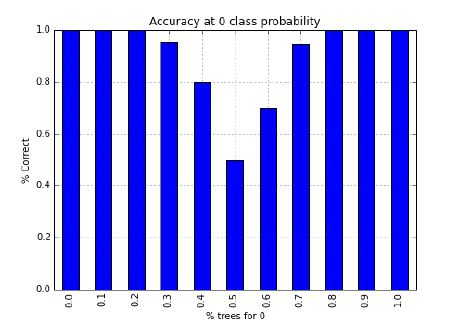
\includegraphics[width=0.7\linewidth]{images/SKL42-RF1}
\caption{}
\label{fig:SKL42-RF1}
\end{figure}

%===================================================%
% % Chapter 4
% % 133
\subsection*{Theoretical Matters}
Random forest works by using a predetermined number of weak Decision Trees and by training
each one of these trees on a subset of data. This is critical in avoiding overfitting. This is also the
reason for the bootstrap parameter. We have each tree trained with the following:

\begin{itemize}
\item  The class with the most votes
\item  The output, if we use regression trees
\end{itemize}
There are, of course, performance considerations, which we'll cover later, but for
the purposes of understanding how random forests work, we train a bunch of average trees
and get a fairly good classifier as a result.
\newpage
\subsection*{Feature Importance}
\begin{itemize}
\item Feature importance is a good by-product of random forests. This often helps to answer the
question: If we have 10 features, which features are most important in determining the true
class of the data point? 
\item The real-world applications are hopefully easy to see.  For example,
if a transaction is fraudulent, we probably want to know if there are certain signals that can
be used to figure out a transaction's class more quickly.
\item If we want to calculate the feature importance, we need to state it when we create the object.
\item \textit{If you use scikit-learn 0.15, you might get a warning that it is not required; in Version 0.16,
the warning will be removed:}
\end{itemize}

\begin{framed}
	\begin{verbatim}
>>> rf = RandomForestClassifier(compute_importances=True)
>>> rf.fit(X, y)
>>> f, ax = plt.subplots(figsize=(7, 5))
>>> ax.bar(range(len(rf.feature_importances_)),
rf.feature_importances_)
>>> ax.set_title("Feature Importances")
\end{verbatim}
\end{framed}
\begin{figure}
\centering
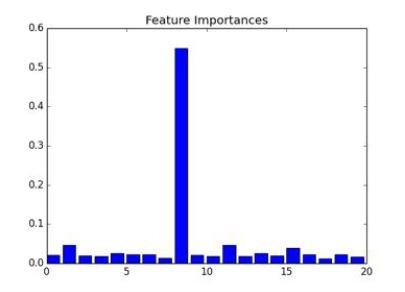
\includegraphics[width=0.7\linewidth]{images/SKL42-RF2}
\caption{}
\label{fig:SKL42-RF2}
\end{figure}

%===================================================%
% % Classifying Data with scikit-learn
% % 134
% The following is the output:
As we can see, certain features are much more important than others when determining if the
outcome was of class 0 or class 1.
\newpage

\section{Tuning a random forest model}
Previously we reviewed how to use the random forest classifier. In this recipe,
we'll walk through how to tune its performance by tuning its parameters.
\subsubsection*{Getting Ready}
In order to tune a random forest model, we'll need to first create a dataset that's a little
more difficult to predict. Then, we'll alter the parameters and do some preprocessing to
fit the dataset better.
So, let's create the dataset first:
\begin{framed}
	\begin{verbatim}
>>> from sklearn import datasets
>>> X, y = datasets.make_classification(n_samples=10000,
n_features=20,
n_informative=15,
flip_y=.5, weights=[.2, .8])
\end{verbatim}
\end{framed}
%===================================================%
% %  Chapter 4
% % 135
\subsection*{Implementation}
we will do the following:
\begin{enumerate}
\item Create a training and test set. 
%We won't just sail through this recipe like we did in
%the previous recipe. It's an empty deed to tune a model without comparing it to a
%training set.
\item Fit a baseline random forest to evaluate how well we do with a naive algorithm.
\item Alter some parameters in a systematic way, and then observe what happens to the fit.
\end{enumerate}
Ok, start an interpreter and import NumPy:
\begin{framed}
	\begin{verbatim}
>>> import numpy as np
>>> training = np.random.choice([True, False], p=[.8, .2],
size=y.shape)
>>> from sklearn.ensemble import RandomForestClassifier
>>> rf = RandomForestClassifier()
>>> rf.fit(X[training], y[training])
>>> preds = rf.predict(X[~training])
>>> print "Accuracy:\t", (preds == y[~training]).mean()
Accuracy: 0.652239557121
\end{verbatim}
\end{framed}
\subsection*{Accuracy}
Accuracy is a good first metric, but using a confusion matrix will help
us understand what's going on.
\begin{itemize}
	\item Accuracy 
	\item Confusion Matrix
\end{itemize}
Let's iterate through the recommended choices for \texttt{max\_features} and see what it does to
the fit. We'll also iterate through a couple of floats, which are the fraction of the features that
will be used. Use the following commands to do so:
\begin{framed}
	\begin{verbatim}
>>> from sklearn.metrics import confusion_matrix
>>> max_feature_params = ['auto', 'sqrt', 'log2', .01, .5, .99]
>>> confusion_matrixes = {}
>>> for max_feature in max_feature_params:
rf = RandomForestClassifier(max_features=max_feature)
\end{verbatim}
\end{framed}
%===================================================%
% % Classifying Data with scikit-learn
% % 136
\begin{framed}
	\begin{verbatim}
rf.fit(X[training], y[training])
>>> confusion_matrixes[max_feature] = confusion_matrix(y[~training])
>>> rf.predict(X[~training])).ravel()
\end{verbatim}
\end{framed}
Since I used the ravel method, our 2D confusion matrices are now 1D.
Now, import pandas and look at the confusion matrix we just created:
\begin{framed}
\begin{verbatim}
>>> import pandas as pd
>>> confusion_df = pd.DataFrame(confusion_matrixes)
>>> import itertools
>>> from matplotlib import pyplot as plt
>>> f, ax = plt.subplots(figsize=(7, 5))
>>> confusion_df.plot(kind='bar', ax=ax)
>>> ax.legend(loc='best')
>>> ax.set_title("Guessed vs Correct (i, j) where i is the guess and j is
the actual.")
>>> ax.grid()
>>> ax.set_xticklabels([str((i, j)) for i, j in
list(itertools.product(range(2), range(2)))]);
>>> ax.set_xlabel("Guessed vs Correct")
>>> ax.set_ylabel("Correct")
\end{verbatim}
\end{framed}
%===================================================%
% % Chapter 4
% % 137
The following is the output:

\begin{itemize}
\item While we didn't see any real difference in performance, this is a fairly simple process to go
through for your own projects. Let's try it on the choice of \texttt{n\_estimator} instances, but use
raw accuracy. 
\item With more than a few options, our graph is going to become very cloudy and
difficult to use.
\item Since we're using the confusion matrix, we can get the accuracy from the trace of the
confusion matrix divided by the overall sum:
\end{itemize}

\begin{framed}
	\begin{verbatim}
>>> n_estimator_params = range(1, 20)
>>> confusion_matrixes = {}
>>> for n_estimator in n_estimator_params:
rf = RandomForestClassifier(n_estimators=n_estimator)
rf.fit(X[training], y[training])
confusion_matrixes[n_estimator] = confusion_matrix(y[~training],
rf.predict(X[~training]))
\end{verbatim}
\end{framed}
%===================================================%
% % Classifying Data with scikit-learn
% % 138
Here's where we'll update the confusion matrix with the
operation we talked about
\begin{framed}
	\begin{verbatim}
>>> accuracy = lambda x: np.trace(x) / np.sum(x, dtype=float)
>>> confusion_matrixes[n_estimator] =
accuracy(confusion_matrixes[n_estimator])
>>> accuracy_series = pd.Series(confusion_matrixes)
>>> import itertools
>>> from matplotlib import pyplot as plt
>>> f, ax = plt.subplots(figsize=(7, 5))
>>> accuracy_series.plot(kind='bar', ax=ax, color='k', alpha=.75)
>>> ax.grid()
>>> ax.set_title("Accuracy by Number of Estimators")
>>> ax.set_ylim(0, 1) # we want the full scope
>>> ax.set_ylabel("Accuracy")
>>> ax.set_xlabel("Number of Estimators")
\end{verbatim}
\end{framed}
The following is the output:
%===================================================%
% % Chapter 4
% % 139
Notice how accuracy is going up for the most part. There certainly is some randomness
associated with the accuracy, but the graph is up and to the right. In the following How it
works... section, we'll talk about the association between random forest and bootstrap,
and what is generally better.

\subsubsection{Bootstrapping}
Bootstrapping is a nice technique to augment the other parts of modeling. The case often used
to introduce bootstrapping is adding standard errors to a median. Here, we just estimate the
outcome over and over and aggregate the estimates up to probabilities.
So, by simply increasing the number estimators, we increase the subsamples that lead to an
overall faster convergence.
There's more…
We might want to speed up the training process. I alluded to this process earlier, but we can
set \texttt{n\_jobs} to the number of trees we want to train at the same time. This should roughly be
the number of cores on the machine:
\begin{framed}
	
\begin{verbatim}
>>> rf = RandomForestClassifier(n_jobs=4, verbose=True)
>>> rf.fit(X, y)
[Parallel(n_jobs=4)]: Done 1 out of 4 | elapsed: 0.3s remaining: 0.9s
[Parallel(n_jobs=4)]: Done 4 out of 4 | elapsed: 0.3s finished
This will also predict in parallel (verbosely):
>>> rf.predict(X)
[Parallel(n_jobs=4)]: Done 1 out of 4 | elapsed: 0.0s remaining:
0.0s
[Parallel(n_jobs=4)]: Done 4 out of 4 | elapsed: 0.0s finished
array([1, 1, 0, ..., 1, 1, 1])
\end{verbatim}
\end{framed}
%===================================================%
% % Classifying Data with scikit-learn
% % 140
\end{document}